\chapter{Implementation} \label{chap:Implementation}


\section{Contribution}

\cite{migliavacca_DADT:2006} presented a prototype that enabled the use of DADTs
to facilitate distributed application programming. While this approach is
clearly applicable to WSNs, the prototype itself did not support WSN
abstractions, and there were several limitations to it:

\begin{itemize}
  \item The lack of a routing mechanism.
  \item Limitations in portability to real WSN nodes.
\end{itemize}

This work makes the following contributions:

\begin{itemize}
  \item Extension of the DADT prototype for use in WSNs by extending it to run
  on simulators as well as devices in a real-world environment.
  \item Interfacing the LN mechanism presented in \cite{mottola_LNAbstraction}
  to enable abstracted communication between groups of nodes in the WSN defined
  by DADTs.
  \item  Verification of the utility of DADT abstractions in the WSN application
  layer.
\end{itemize}

\section{The DADT/LN Architecture}

% FILL THIS IN LATER.
\subsection{Overview}
\begin{figure}
\centering
\label{Fig:DADTLN_architecture}
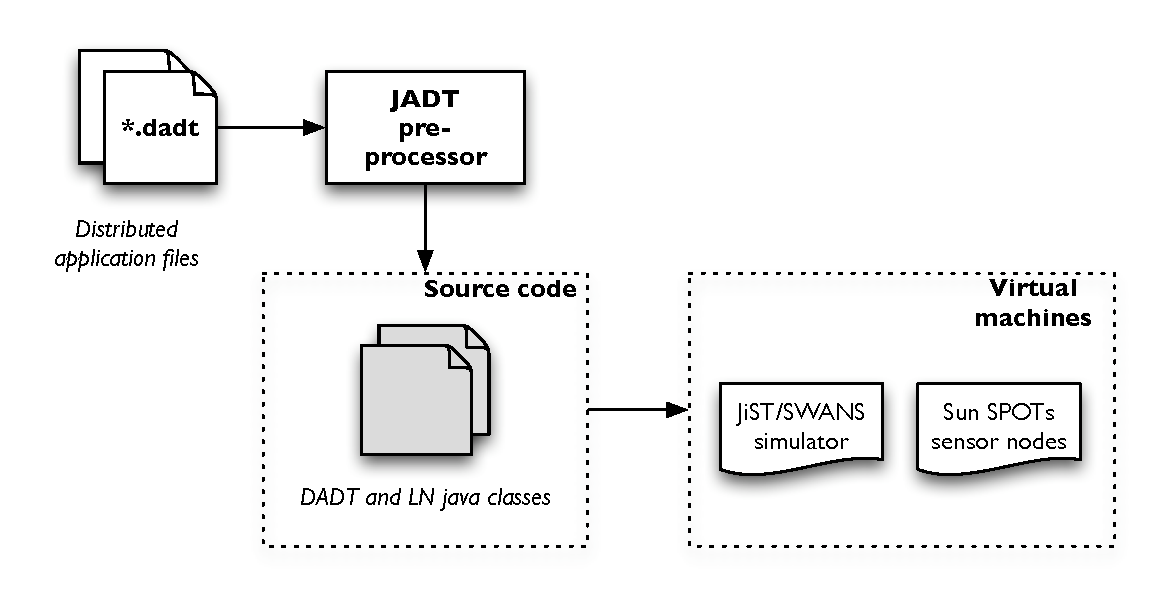
\includegraphics[scale=0.71]{img/DADTLN_architecture.eps} \caption[DADT/LN
application workflow]{Workflow for development of an application that uses
the DADT/LN prototype}
\end{figure} 
The overview of the workflow involved in using DADTs to enable WSN application
programming is as shown in Figure \ref{Fig:DADTLN_architecture}. The user writes
application layer code for the WSN using a DADT language in a series of
\emph{.dadt} files. A preprocessor is used to convert the code written by the
application programmer into Java code that interfaces with the DADT
infrastructure (extended from the prototype presented in
\cite{migliavacca_DADT:2006}). In order to facilitate routing to LNs defined by
the use of DADT views, the DADT infrastructure is interfaced with the a
previously developed implementation of LNs. 

The application (including the implementation of layers lower in the protocol
stack) is then loaded on to either:
\begin{itemize}
\item the JiST/SWANS simulator \cite{barr_JIST:2005, barr_SWANS}. See Section \ref{sec:jistswans} for details on the implementation of
the aforementioned simulator
\item a collection of Sun SPOT wireless sensor devices \cite{simon_squawk:2006}
(see Section \ref{sec:sunspots}) to execute the application on real sensor nodes.
\end{itemize}

\subsection{Execution Details}

This section outlines the communication mechanisms used for the development and
execution of an application that uses the DADT/LN architecture developed as part
of this work.



\section{Simulation using JiST/SWANS}

\section{DADT-LN on Sun SPOTs}

\section{Challenges}

\section{Future Work}

\section{Evaluation}

\section{Analysis of Results}

